%
% File acl2020.tex
%
%% Based on the style files for ACL 2020, which were
%% Based on the style files for ACL 2018, NAACL 2018/19, which were
%% Based on the style files for ACL-2015, with some improvements
%%  taken from the NAACL-2016 style
%% Based on the style files for ACL-2014, which were, in turn,
%% based on ACL-2013, ACL-2012, ACL-2011, ACL-2010, ACL-IJCNLP-2009,
%% EACL-2009, IJCNLP-2008...
%% Based on the style files for EACL 2006 by 
%%e.agirre@ehu.es or Sergi.Balari@uab.es
%% and that of ACL 08 by Joakim Nivre and Noah Smith

\documentclass[11pt,a4paper]{article}
\usepackage[hyperref]{acl2020}
\usepackage{times}
\usepackage{latexsym}
\renewcommand{\UrlFont}{\ttfamily\small}

% This is not strictly necessary, and may be commented out,
% but it will improve the layout of the manuscript,
% and will typically save some space.
\usepackage{microtype}

%\aclfinalcopy % Uncomment this line for the final submission
%\def\aclpaperid{***} %  Enter the acl Paper ID here

%\setlength\titlebox{5cm}
% You can expand the titlebox if you need extra space
% to show all the authors. Please do not make the titlebox
% smaller than 5cm (the original size); we will check this
% in the camera-ready version and ask you to change it back.

\usepackage{subfigure}
\usepackage{tikz}
\usetikzlibrary{arrows,positioning,fit,shapes}

\newcommand\BibTeX{B\textsc{ib}\TeX}

\title{How much of enhanced UD is contained in UD?}
% How enhanced is enhanced UD?

\author{First Author \\
  Affiliation / Address line 1 \\
  Affiliation / Address line 2 \\
  Affiliation / Address line 3 \\
  \texttt{email@domain} \\\And
  Second Author \\
  Affiliation / Address line 1 \\
  Affiliation / Address line 2 \\
  Affiliation / Address line 3 \\
  \texttt{email@domain} \\}

\date{}

\begin{document}
\maketitle
\begin{abstract}
  TODO
\end{abstract}

\section{Introduction}
(ADAM)

In this paper we present an approach to producing enhanced universal
dependencies.

General idea: as described by the website
(https://universaldependencies.org/u/overview/enhanced-syntax.html)
for many cases, enhanced UD is a function of UD.

Hypothesis: most information about EUD is already contained in UD.

Describe task again.

What is ELAS and EULAS  score.

Implement the function for the common case, and see how we fare on the
ELAS and EULAS  score.

Results in 2 lines:
- scores
- efficient
- transparent

\section{Method}


In essence, our method is to apply the recipes provided by TODO to
transform UD \emph{trees} into EUD graphs.

To do so, we use a tree-matching procedure against a UD tree, and
locally insert (and sometimes delete) edges. As a particular case, we
may re-label some edges.

Perhaps surprisingly, the patterns that we need to recognize are
pretty simple, involving only three nodes. The patterns are listed in
TODO.


match tree patterns which call for enhancing of the

dependency structure. We identify 2 types of paterns.

(ADAM) Insert figure:

``Paul and Mary eat.''
``She was reading or watching something''

\begin{figure}
\centering
\begin{subfigure}[b]{0.5cm}
  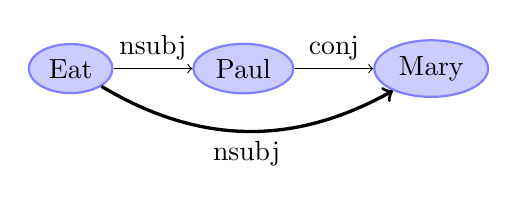
\begin{tikzpicture}[inner sep=1mm,
    word/.style={ellipse,draw=blue!50,fill=blue!20,thick}]
    \node[word] (eat) {Eat};
    \node[word] (paul) [right=of eat] {Paul};
    \node[word] (mary) [right=of paul] {Mary};
    \draw[->] (eat) -- node[above] {nsubj} (paul);
    \draw[->] (paul) -- node[above] {conj} (mary);
    \path (eat) edge[->,very thick,bend right]  node[below] {nsubj} (mary);
  \end{tikzpicture}
  \caption{Relation pointing to the conjuncts}
\end{subfigure}

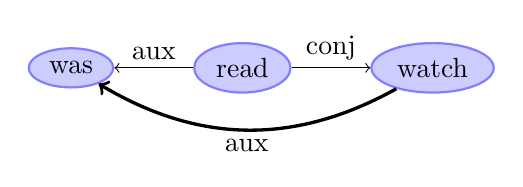
\begin{tikzpicture}[inner sep=1mm,
  word/.style={ellipse,draw=blue!50,fill=blue!20,thick}]
  \node[word] (was) {was};
  \node[word] (read) [right=of was] {read};
  \node[word] (watch) [right=of read] {watch};
  \draw[->] (read) -- node[above] {aux} (was);
  \draw[->] (read) -- node[above] {conj} (watch);
  \path (watch) edge[->,very thick,bend left]  node[below] {aux} (was);
\end{tikzpicture}

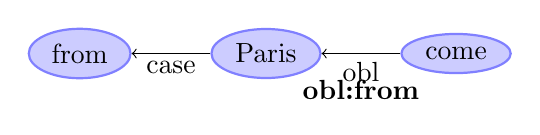
\begin{tikzpicture}[inner sep=1mm,
  word/.style={ellipse,draw=blue!50,fill=blue!20,thick}]
  \node[word] (from) {from};
  \node[word] (paris) [right=of from] {Paris};
  \node[word] (come) [right=of paris] {come};
  \draw[->] (paris) -- node[below] {case} (from);
  \draw[->] (come) -- node[below] (lab) {obl} (paris);
  \node at (lab.south) {\textbf{obl:from}};
\end{tikzpicture}

\caption{Transformation patterns. Added elements are shown in bold.}
  \label{fig:patterns}
\end{figure}

Extensions:
- deletion of arrows

- finding label names


Adam: figure for this:

John came from Paris




Missing cases:


\section{Results}
(ADAM)

\begin{table}[h]
	\centering
	\begin{tabular}{l|rr}
		\textsc{Language} & \textsc{ELAS} & \textsc{EULAS} \\
		\hline
		Arabic &  & \\
		Bulgarian &  & \\
		Czech &  & \\
		Dutch &  & \\
		English &  & \\
		Estonian &  & \\
		Finnish &  & \\
		French &  & \\
		Italian &  & \\
		Latvian &  & \\
		Lithuanian &  & \\
		Polish &  & \\
		Russian &  & \\
		Slovak &  & \\
		Swedish &  & \\
		Tamil &  & \\
		Ukrainian &  & \\
		Average &  & \\
	\end{tabular}
\caption{Test set results}
\end{table}

\begin{table}[h]
	\centering
	\begin{tabular}{l|rr}
		\textsc{Language} & \textsc{ELAS} & \textsc{EULAS} \\
		\hline 
		Arabic &  & \\
		Bulgarian &  & \\
		Czech &  & \\
		Dutch &  & \\
		English &  & \\
		Estonian &  & \\
		Finnish &  & \\
		French &  & \\
		Italian &  & \\
		Latvian &  & \\
		Lithuanian &  & \\
		Polish &  & \\
		Russian &  & \\
		Slovak &  & \\
		Swedish &  & \\
		Tamil &  & \\
		Ukrainian &  & \\
		Average &  & \\ 
	\end{tabular}
	\caption{Gold tree results}
\end{table} 
TODO: Add std dev.

TODO: what is the baseline (just deleting enhanced dependencies from the gold files)?

\section{Discussion/Analysis}
(JP)

It works!

Labels work for english but not well for all languages.

Secondary hyp: EUD do not help for learning EUD.

We do not know about this YET. For this we'd need to use compare a
state of art UD implementation.


To test that we'd need to run our system on the \emph{training} data
of a state of the art EUD system and see how that affects its
performance. But we can't do it since such systems are not available
yet (this is the purpose of the task ...).

Also can be used for bootstrapping.

\section*{Acknowledgments}

(Anonymized)

\bibliography{anthology,acl2020}
\bibliographystyle{acl_natbib}


\end{document}
